In this chapter, simulations are carried out to verify the swarm algorithm design and implementation.
Firstly, the simulation bed is introduced,
which is a simulation platform developed as a part of this project.
Then, the results of two simulation cases are presented and analysed.
Lastly, the swarm algorithm and the implementation are evaluated based on the simulations.

\section{The Simulation Bed}

There are already existing simulation platforms for testing UAV swarms \parencite{Chen2023}.
However, most of these platforms are too complex
and not suitable for the specific problem stated in chapter \ref{chap_problem}.
Hence, a simple but sufficient simulation bed is developed.

During a simulation of an $N$-sized swarm,
there will be $N+1$ processes, as shown in figure \ref{fig:simbed}.
$N$ processes are for the $N$ UAVs, and the remaining one is for the simulation bed.
Currently, all the processes are single-threaded.
Each UAV process executes a copy of the onboard software implemented in chapter \ref{chap_impl},
with its own UAV-specific arguments such as its unique UAV ID.
The simulation bed process communicates with the UAV processes through non-blocking Unix sockets.
The main functionalities of the simulation bed are as follows.
\begin{itemize}
    \item Receiving the velocity values set by a UAV, carrying out kinematic integration,
          and sending the calculated positions back to the UAV.
    \item Collecting the messages sent by the UAVs
          and dispatching the messages to their recipient UAVs.
    \item Detecting collisions and removing crashed UAVs.
    \item Sending GCS tasks to the swarm.
    \item Dumping the states of the UAVs periodically to an output file.
\end{itemize}

\begin{figure}[htbp]
  \centering
  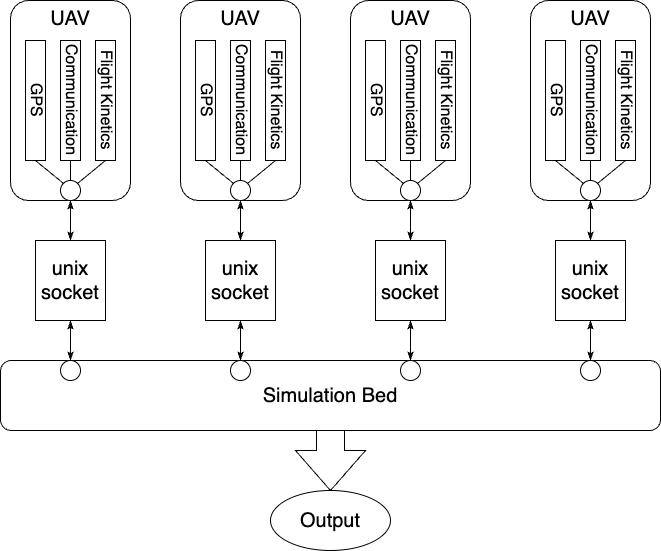
\includegraphics[width=0.8\linewidth]{rsc/simbed.png}
  \caption[Simulation bed.]
  {UAV processes and the simulation bed process.}
  \label{fig:simbed}
\end{figure}

\section{Simulation Results}
\label{sec:sim_res}

In the simulations in this section, the radius of a UAV is $0.1m$,
which is similar to the size of a DJI Mini 2 \parencite{DJI2024} drone.
The maximum speed of a UAV is $4m/s$.
The communication range of a UAV is $30m$.
In each simulation case, 10 seconds after the start of the simulation,
a task will be sent by the simulation bed to 1 or 2 of the UAVs.

\subsection{Simple Line Task}

In this case, 10 UAVs are commanded to form a straight line
from point $(0m, 10m, 10m)$ to point $(0m, 20m, 10m)$.
Figure \ref{fig:sim_line_001} to \ref{fig:sim_line_220} show
the swarm organisation process and the task execution process.

In figure \ref{fig:sim_line_001}, at simulation time $0.1s$,
10 UAVs are at their initial positions, each of them being a separate single-node swarm.
Figure \ref{fig:sim_line_020} and figure \ref{fig:sim_line_040} show
the UAVs organise themselves into a single swarm after some attempts.
The tree structure plots are based on the NIDs of the UAVs.
During the swarm organisation process, tree-switching algorithm is executed.
The NIDs of UAVs may change constantly,
until stable connections are established between all child-parent pairs.

Figure \ref{fig:sim_line_140} to \ref{fig:sim_line_220} show
the UAVs fly onto the designated line after receiving the task.
Each UAV occupies a different point of the line.
UAVs coordinate with each other to form the whole line.

This simulation case demonstrates that
the swarm algorithm and the implementation perform as designed.
Both swarm control and task coordination are accomplished successfully.

\begin{figure}[htbp]
  \centering
  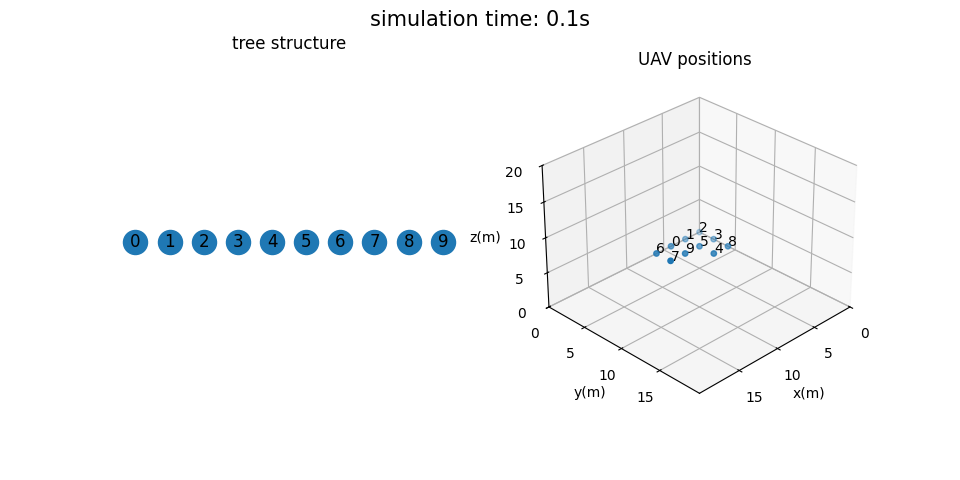
\includegraphics[width=0.96\linewidth]{rsc/line.01.png}
  \caption{Line task at 0.1s.}
  \label{fig:sim_line_001}
\end{figure}

\begin{figure}[htbp]
  \centering
  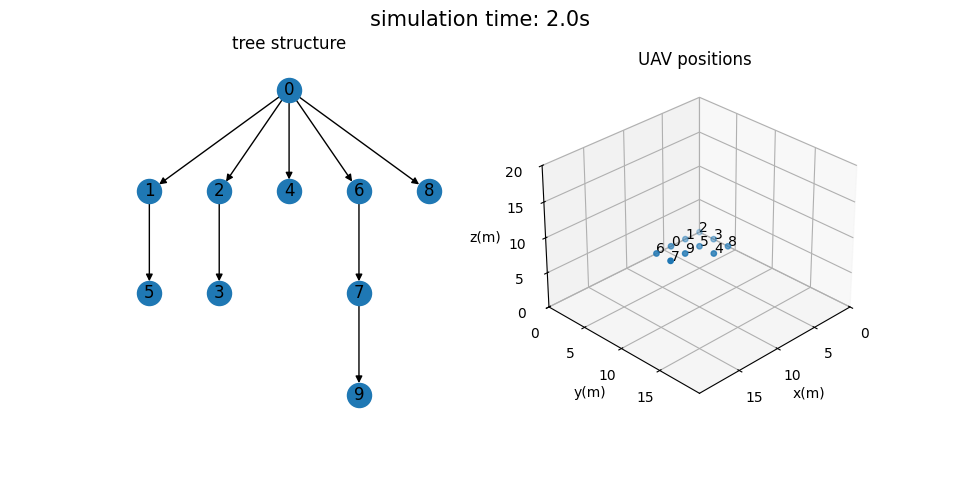
\includegraphics[width=0.96\linewidth]{rsc/line.05.png}
  \caption{Line task at 2.0s.}
  \label{fig:sim_line_020}
\end{figure}

\begin{figure}[htbp]
  \centering
  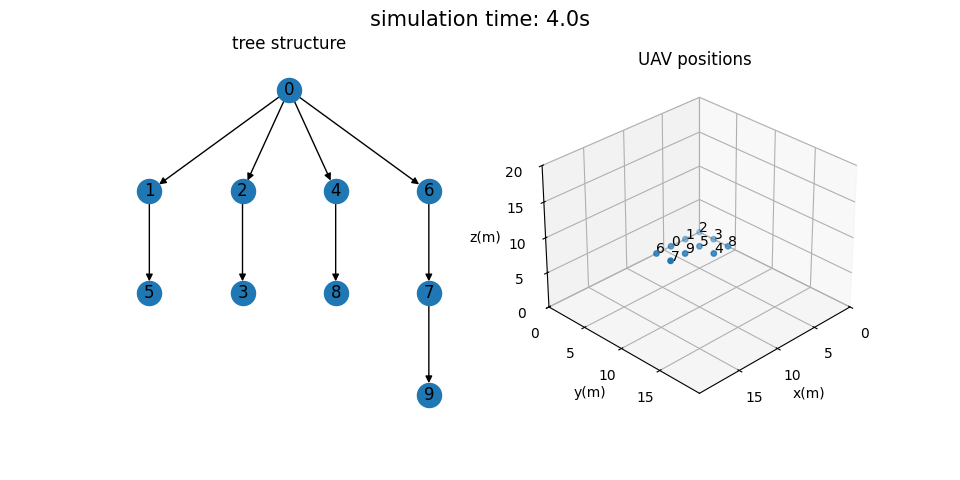
\includegraphics[width=0.96\linewidth]{rsc/line.06.png}
  \caption{Line task at 4.0s.}
  \label{fig:sim_line_040}
\end{figure}

\begin{figure}[htbp]
  \centering
  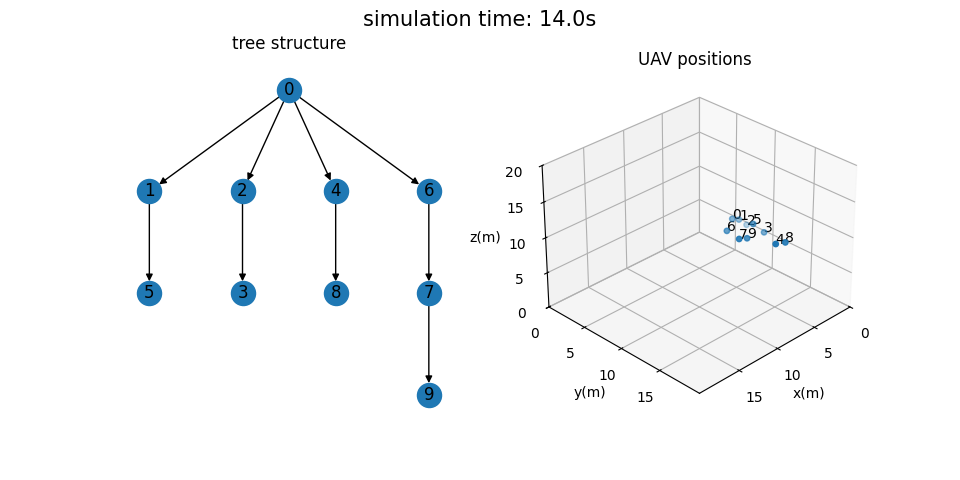
\includegraphics[width=0.96\linewidth]{rsc/line.11.png}
  \caption{Line task at 14.0s.}
  \label{fig:sim_line_140}
\end{figure}

\begin{figure}[htbp]
  \centering
  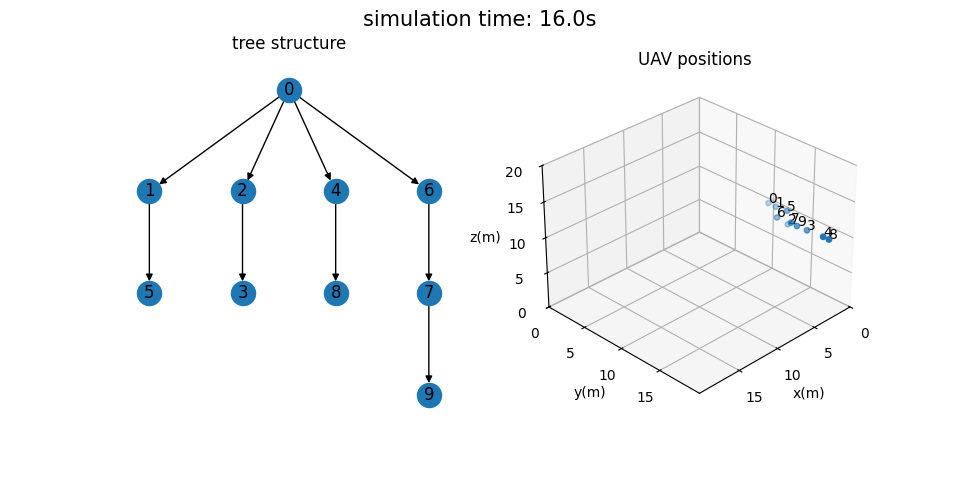
\includegraphics[width=0.96\linewidth]{rsc/line.12.png}
  \caption{Line task at 16.0s.}
  \label{fig:sim_line_160}
\end{figure}

\begin{figure}[htbp]
  \centering
  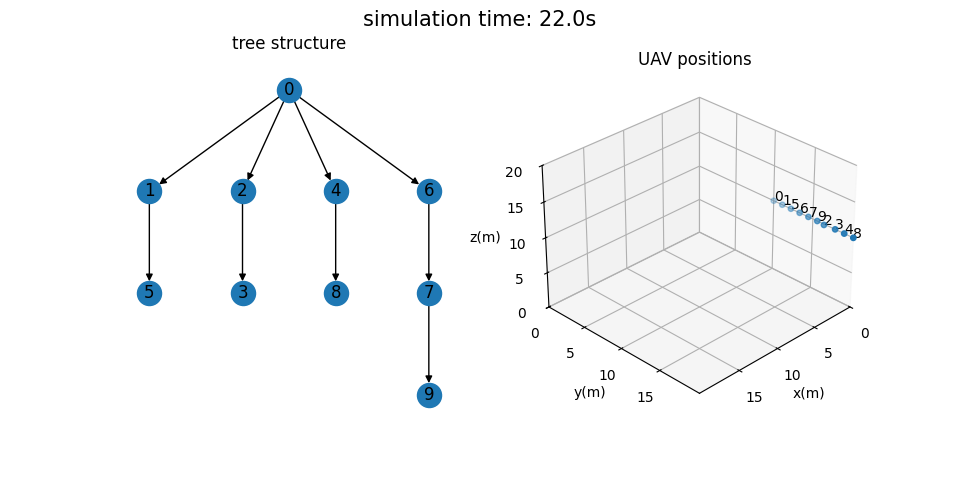
\includegraphics[width=0.96\linewidth]{rsc/line.15.png}
  \caption{Line task at 22.0s.}
  \label{fig:sim_line_220}
\end{figure}

\subsection{Letter Task}

In this case, 50 UAVs are commanded to form the letters ``LOVE".

Figure \ref{fig:sim_lttr_001} to \ref{fig:sim_lttr_080} show the swarm organisation process.
Compared to the simple line task, due to a much large swarm size,
it takes the UAVs more time to establish a stable tree structure.
The resulted tree is also more complicated.

Figure \ref{fig:sim_lttr_160} to \ref{fig:sim_lttr_280} show the task execution process.
This letter task is comprised of multiple lines. Moreover, the letter `O' is a curve.
The success of this task proves the effectiveness of the task division algorithm.

This simulation case demonstrates that
the swarm algorithm is suitable for a large swarm to handle complex tasks.

\begin{figure}[htbp]
  \centering
  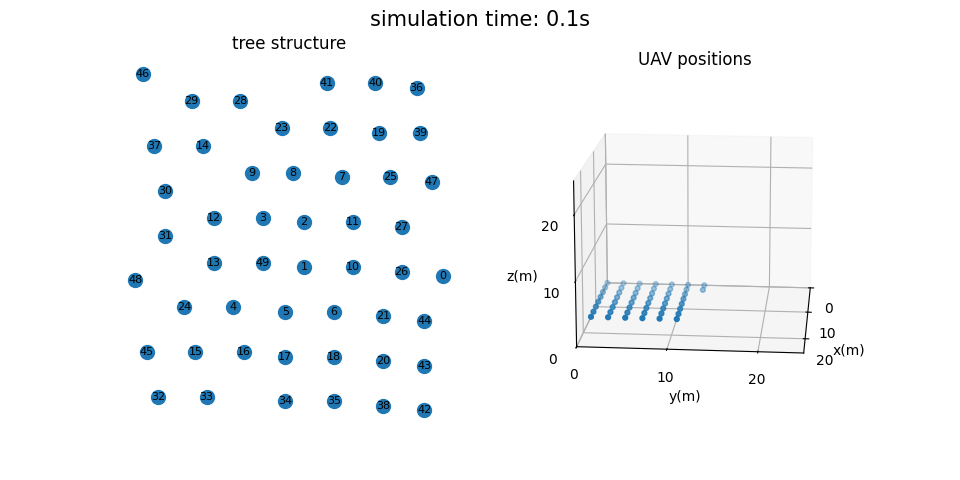
\includegraphics[width=0.96\linewidth]{rsc/lttr.01.png}
  \caption{Letter task at 0.1s.}
  \label{fig:sim_lttr_001}
\end{figure}

\begin{figure}[htbp]
  \centering
  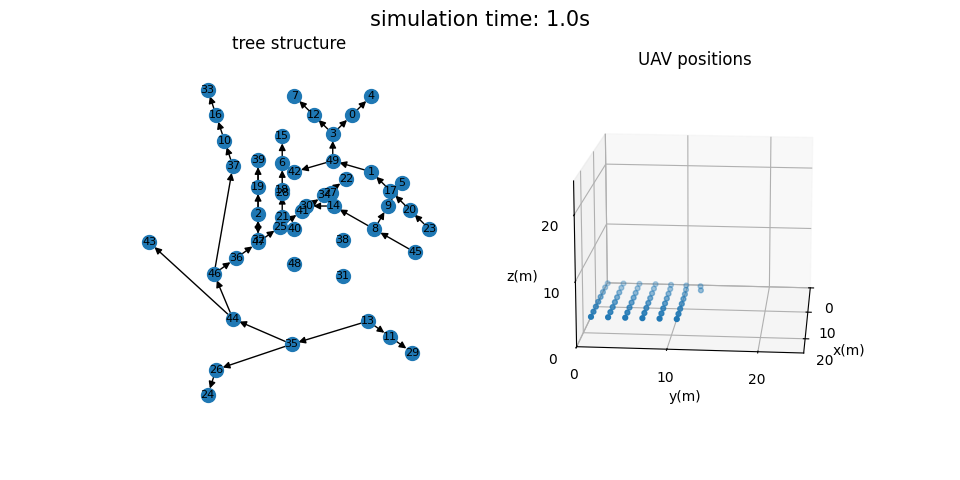
\includegraphics[width=0.96\linewidth]{rsc/lttr.04.png}
  \caption{Letter task at 1.0s.}
  \label{fig:sim_lttr_010}
\end{figure}

\begin{figure}[htbp]
  \centering
  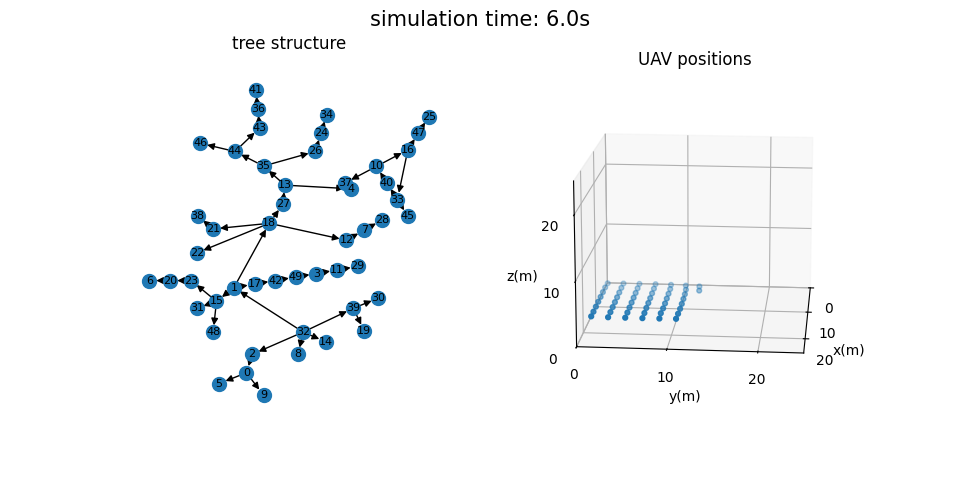
\includegraphics[width=0.96\linewidth]{rsc/lttr.07.png}
  \caption{Letter task at 6.0s.}
  \label{fig:sim_lttr_060}
\end{figure}

\begin{figure}[htbp]
  \centering
  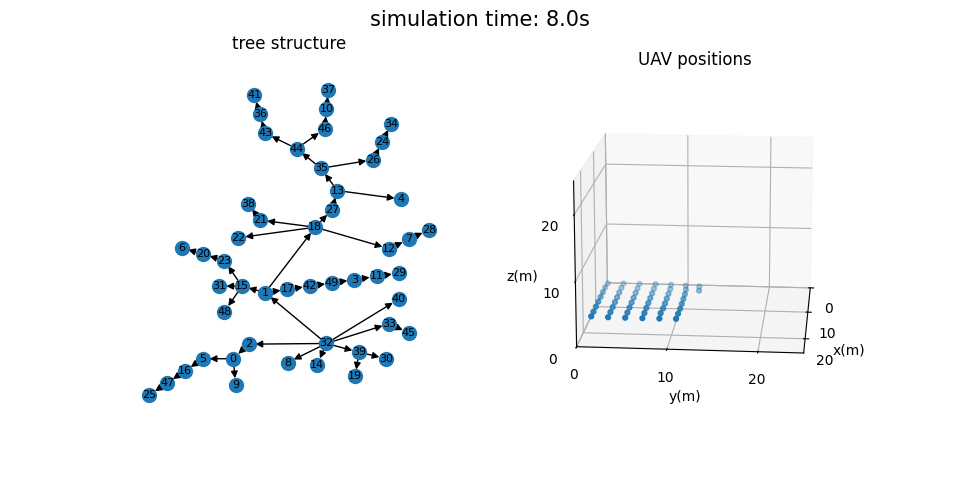
\includegraphics[width=0.96\linewidth]{rsc/lttr.08.png}
  \caption{Letter task at 8.0s.}
  \label{fig:sim_lttr_080}
\end{figure}

\begin{figure}[htbp]
  \centering
  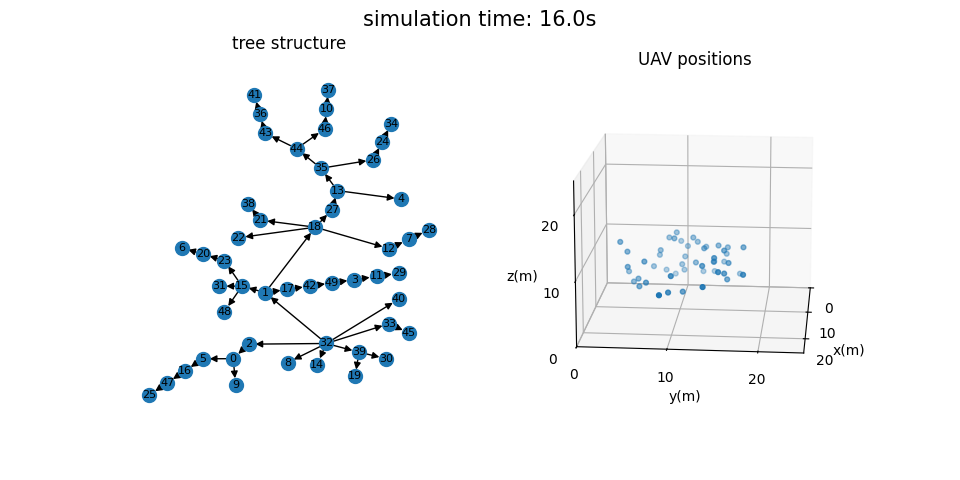
\includegraphics[width=0.96\linewidth]{rsc/lttr.12.png}
  \caption{Letter task at 16.0s.}
  \label{fig:sim_lttr_160}
\end{figure}

\begin{figure}[htbp]
  \centering
  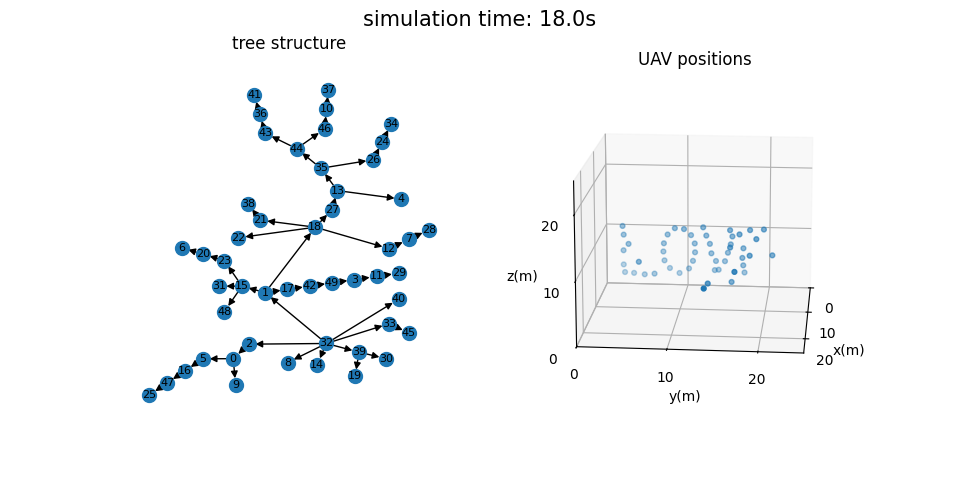
\includegraphics[width=0.96\linewidth]{rsc/lttr.13.png}
  \caption{Letter task at 18.0s.}
  \label{fig:sim_lttr_180}
\end{figure}

\begin{figure}[htbp]
  \centering
  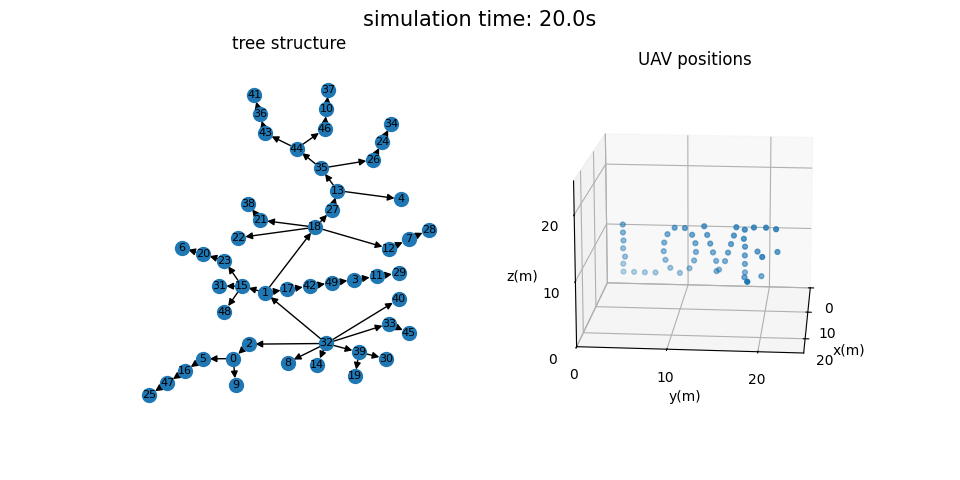
\includegraphics[width=0.96\linewidth]{rsc/lttr.14.png}
  \caption{Letter task at 20.0s.}
  \label{fig:sim_lttr_200}
\end{figure}

\begin{figure}[htbp]
  \centering
  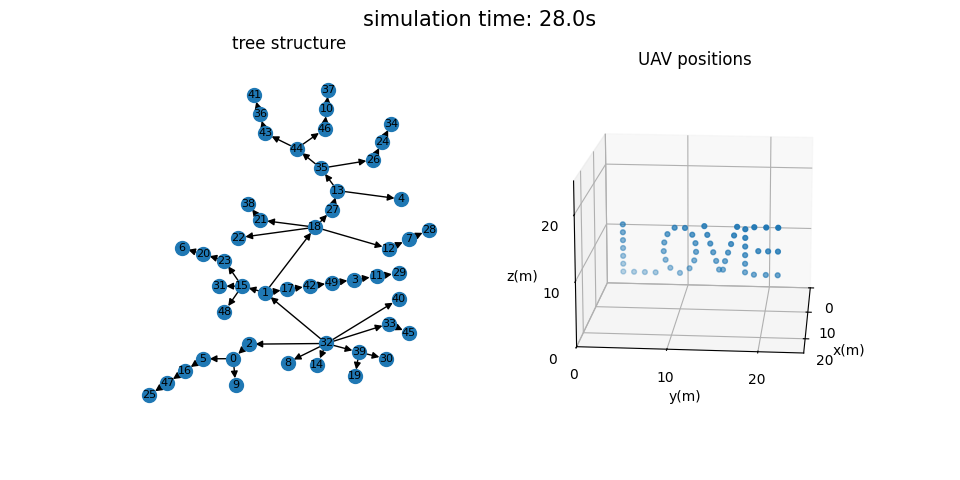
\includegraphics[width=0.96\linewidth]{rsc/lttr.18.png}
  \caption{Letter task at 28.0s.}
  \label{fig:sim_lttr_280}
\end{figure}

\section{Evaluation}
\label{sec:eval}

The simulation results in section \ref{sec:sim_res} show that
the problem in chapter \ref{chap_problem} is successfully solved.
The design of the swarm algorithm in chapter \ref{chap_design} is demonstrated,
and the implementation in chapter \ref{chap_impl} is validated.
It can be seen that a group of UAVs can dynamically organise themselves into a tree structure.
UAVs in such hierarchical swarm can coordinate with each other to carry out tasks.
A task is divided layer by layer down the tree,
with each UAV responsible for its own part of the task.

This thesis is inspired by drone shows.
The overall goal of this thesis is successfully achieved,
and the results indicate the potential usage of autonomous swarms in future drone shows.
However, there are still a lot of problems to be addressed.
\begin{itemize}
    \item Support for very large swarm sizes (>100) needs to be verified.
          One of the reasons of the hierarchical design is to support extremely large swarm sizes.
          However, the simulation bed in this thesis involves a lot of inter-process communication,
          which is time-consuming and limits the maximum simulated swarm size.
    \item Support for limited communication range needs to be tested.
          In the simulations in section \ref{sec:sim_res},
          the communication range is large enough
          so that two arbitrary UAVs can communicate with each other.
          But in the design, a UAV does not have to be able to communicate with all the other UAVs.
          Simulation cases are needed where the communication range does not cover the whole swarm.
          The shape division algorithm in section \ref{sec:tsk_div} also needs to be adapted
          if the communication range does not cover the whole shape.
    \item The tree structure of a swarm is not optimised.
          The current design only ensures the swarm is organised into a tree,
          but does not ensure the tree structure is optimal.
          To improve the communication and coordination inside the swarm,
          the tree should be as balanced as possible.
          It should not be too deep.
          Nor should parent nodes have too many children.
          So some kind of optimisation algorithm is needed.
    \item There is no fault tolerance and fault recovery for task execution.
          The dynamic tree organisation design solves the fault tolerance problem
          when the swarm is in free state.
          But during task execution, in the current implementation,
          if any single UAV fails, the whole task fails.
          This compromises the robustness of the swarm.
\end{itemize}
Apart from the above problems,
the following aspects which are ignored in this thesis
also restrain the application of the swarm algorithm in any real drone shows.
\begin{itemize}
    \item Lack of obstacle detection.
          UAVs are not able to detect obstacles and other UAVs.
          They acquire the positions of other UAVs through receiving broadcasting messages.
          Broadcasting frequency must be high to reduce the possibility of collisions.
          But frequent broadcasting leads to high performance overhead.
    \item Lack of the ability to deal with complex or animated patterns.
          In real drone shows, the patterns are more than just simple shapes.
          Patterns may also transform smoothly from one into another.
    \item Other problems such as no battery management, no LED lights control,
          unrealistic flight kinetics, etc.
\end{itemize}